% Options for packages loaded elsewhere
\PassOptionsToPackage{unicode}{hyperref}
\PassOptionsToPackage{hyphens}{url}
%
\documentclass[
]{article}
\usepackage{lmodern}
\usepackage{amssymb,amsmath}
\usepackage{ifxetex,ifluatex}
\ifnum 0\ifxetex 1\fi\ifluatex 1\fi=0 % if pdftex
  \usepackage[T1]{fontenc}
  \usepackage[utf8]{inputenc}
  \usepackage{textcomp} % provide euro and other symbols
\else % if luatex or xetex
  \usepackage{unicode-math}
  \defaultfontfeatures{Scale=MatchLowercase}
  \defaultfontfeatures[\rmfamily]{Ligatures=TeX,Scale=1}
\fi
% Use upquote if available, for straight quotes in verbatim environments
\IfFileExists{upquote.sty}{\usepackage{upquote}}{}
\IfFileExists{microtype.sty}{% use microtype if available
  \usepackage[]{microtype}
  \UseMicrotypeSet[protrusion]{basicmath} % disable protrusion for tt fonts
}{}
\makeatletter
\@ifundefined{KOMAClassName}{% if non-KOMA class
  \IfFileExists{parskip.sty}{%
    \usepackage{parskip}
  }{% else
    \setlength{\parindent}{0pt}
    \setlength{\parskip}{6pt plus 2pt minus 1pt}}
}{% if KOMA class
  \KOMAoptions{parskip=half}}
\makeatother
\usepackage{xcolor}
\IfFileExists{xurl.sty}{\usepackage{xurl}}{} % add URL line breaks if available
\IfFileExists{bookmark.sty}{\usepackage{bookmark}}{\usepackage{hyperref}}
\hypersetup{
  pdftitle={COVID-19 Analysis in South Korea},
  pdfauthor={Group 86 - Jana Schneider, Jana Jeggle, Felix Heim, Leon Gaertner},
  hidelinks,
  pdfcreator={LaTeX via pandoc}}
\urlstyle{same} % disable monospaced font for URLs
\usepackage[margin=1in]{geometry}
\usepackage{color}
\usepackage{fancyvrb}
\newcommand{\VerbBar}{|}
\newcommand{\VERB}{\Verb[commandchars=\\\{\}]}
\DefineVerbatimEnvironment{Highlighting}{Verbatim}{commandchars=\\\{\}}
% Add ',fontsize=\small' for more characters per line
\usepackage{framed}
\definecolor{shadecolor}{RGB}{248,248,248}
\newenvironment{Shaded}{\begin{snugshade}}{\end{snugshade}}
\newcommand{\AlertTok}[1]{\textcolor[rgb]{0.94,0.16,0.16}{#1}}
\newcommand{\AnnotationTok}[1]{\textcolor[rgb]{0.56,0.35,0.01}{\textbf{\textit{#1}}}}
\newcommand{\AttributeTok}[1]{\textcolor[rgb]{0.77,0.63,0.00}{#1}}
\newcommand{\BaseNTok}[1]{\textcolor[rgb]{0.00,0.00,0.81}{#1}}
\newcommand{\BuiltInTok}[1]{#1}
\newcommand{\CharTok}[1]{\textcolor[rgb]{0.31,0.60,0.02}{#1}}
\newcommand{\CommentTok}[1]{\textcolor[rgb]{0.56,0.35,0.01}{\textit{#1}}}
\newcommand{\CommentVarTok}[1]{\textcolor[rgb]{0.56,0.35,0.01}{\textbf{\textit{#1}}}}
\newcommand{\ConstantTok}[1]{\textcolor[rgb]{0.00,0.00,0.00}{#1}}
\newcommand{\ControlFlowTok}[1]{\textcolor[rgb]{0.13,0.29,0.53}{\textbf{#1}}}
\newcommand{\DataTypeTok}[1]{\textcolor[rgb]{0.13,0.29,0.53}{#1}}
\newcommand{\DecValTok}[1]{\textcolor[rgb]{0.00,0.00,0.81}{#1}}
\newcommand{\DocumentationTok}[1]{\textcolor[rgb]{0.56,0.35,0.01}{\textbf{\textit{#1}}}}
\newcommand{\ErrorTok}[1]{\textcolor[rgb]{0.64,0.00,0.00}{\textbf{#1}}}
\newcommand{\ExtensionTok}[1]{#1}
\newcommand{\FloatTok}[1]{\textcolor[rgb]{0.00,0.00,0.81}{#1}}
\newcommand{\FunctionTok}[1]{\textcolor[rgb]{0.00,0.00,0.00}{#1}}
\newcommand{\ImportTok}[1]{#1}
\newcommand{\InformationTok}[1]{\textcolor[rgb]{0.56,0.35,0.01}{\textbf{\textit{#1}}}}
\newcommand{\KeywordTok}[1]{\textcolor[rgb]{0.13,0.29,0.53}{\textbf{#1}}}
\newcommand{\NormalTok}[1]{#1}
\newcommand{\OperatorTok}[1]{\textcolor[rgb]{0.81,0.36,0.00}{\textbf{#1}}}
\newcommand{\OtherTok}[1]{\textcolor[rgb]{0.56,0.35,0.01}{#1}}
\newcommand{\PreprocessorTok}[1]{\textcolor[rgb]{0.56,0.35,0.01}{\textit{#1}}}
\newcommand{\RegionMarkerTok}[1]{#1}
\newcommand{\SpecialCharTok}[1]{\textcolor[rgb]{0.00,0.00,0.00}{#1}}
\newcommand{\SpecialStringTok}[1]{\textcolor[rgb]{0.31,0.60,0.02}{#1}}
\newcommand{\StringTok}[1]{\textcolor[rgb]{0.31,0.60,0.02}{#1}}
\newcommand{\VariableTok}[1]{\textcolor[rgb]{0.00,0.00,0.00}{#1}}
\newcommand{\VerbatimStringTok}[1]{\textcolor[rgb]{0.31,0.60,0.02}{#1}}
\newcommand{\WarningTok}[1]{\textcolor[rgb]{0.56,0.35,0.01}{\textbf{\textit{#1}}}}
\usepackage{graphicx}
\makeatletter
\def\maxwidth{\ifdim\Gin@nat@width>\linewidth\linewidth\else\Gin@nat@width\fi}
\def\maxheight{\ifdim\Gin@nat@height>\textheight\textheight\else\Gin@nat@height\fi}
\makeatother
% Scale images if necessary, so that they will not overflow the page
% margins by default, and it is still possible to overwrite the defaults
% using explicit options in \includegraphics[width, height, ...]{}
\setkeys{Gin}{width=\maxwidth,height=\maxheight,keepaspectratio}
% Set default figure placement to htbp
\makeatletter
\def\fps@figure{htbp}
\makeatother
\setlength{\emergencystretch}{3em} % prevent overfull lines
\providecommand{\tightlist}{%
  \setlength{\itemsep}{0pt}\setlength{\parskip}{0pt}}
\setcounter{secnumdepth}{-\maxdimen} % remove section numbering
\ifluatex
  \usepackage{selnolig}  % disable illegal ligatures
\fi

\title{COVID-19 Analysis in South Korea}
\author{Group 86 - Jana Schneider, Jana Jeggle, Felix Heim, Leon
Gaertner}
\date{4 12 2020}

\begin{document}
\maketitle

~

\begin{Shaded}
\begin{Highlighting}[]
\CommentTok{\#general libraries}
\KeywordTok{library}\NormalTok{(magrittr)}
\KeywordTok{library}\NormalTok{(data.table)}
\KeywordTok{library}\NormalTok{(ggplot2)}
\KeywordTok{library}\NormalTok{(tidyr)}
\KeywordTok{library}\NormalTok{(dplyr)}
\KeywordTok{library}\NormalTok{(ggpubr)}
\CommentTok{\#required libraries for Claim 1}
\KeywordTok{library}\NormalTok{(patchwork)}
\KeywordTok{library}\NormalTok{(hrbrthemes)}
\CommentTok{\#required libraries for Claim 3}
\KeywordTok{library}\NormalTok{(maps)}
\KeywordTok{library}\NormalTok{(ggrepel)}
\KeywordTok{library}\NormalTok{(rgeos)}
\KeywordTok{library}\NormalTok{(sf)}
\KeywordTok{library}\NormalTok{(rnaturalearth)}
\KeywordTok{library}\NormalTok{(rnaturalearthdata)}
\end{Highlighting}
\end{Shaded}

\begin{Shaded}
\begin{Highlighting}[]
\CommentTok{\#import data files}
\NormalTok{time \textless{}{-}}\StringTok{ }\KeywordTok{fread}\NormalTok{(}\StringTok{"./extData/Time.csv"}\NormalTok{)}
\NormalTok{policy \textless{}{-}}\StringTok{ }\KeywordTok{fread}\NormalTok{(}\StringTok{"./extData/Policy.csv"}\NormalTok{)}
\NormalTok{policy1 \textless{}{-}}\StringTok{ }\KeywordTok{fread}\NormalTok{(}\StringTok{"./extData/Policy.csv"}\NormalTok{)}
\NormalTok{RKI\_data \textless{}{-}}\StringTok{ }\KeywordTok{fread}\NormalTok{(}\StringTok{"./extData/DE\_InfectionCases.csv"}\NormalTok{)}
\NormalTok{patientinfo \textless{}{-}}\StringTok{ }\KeywordTok{fread}\NormalTok{(}\StringTok{"./extData/PatientInfo.csv"}\NormalTok{)}
\NormalTok{case \textless{}{-}}\StringTok{ }\KeywordTok{fread}\NormalTok{(}\StringTok{"./extData/Case.csv"}\NormalTok{)}
\NormalTok{searchtrend \textless{}{-}}\StringTok{ }\KeywordTok{fread}\NormalTok{(}\StringTok{"./extData/SearchTrend.csv"}\NormalTok{)}
\NormalTok{region \textless{}{-}}\StringTok{ }\KeywordTok{fread}\NormalTok{(}\StringTok{"./extData/Region.csv"}\NormalTok{)}
\end{Highlighting}
\end{Shaded}

~

\hypertarget{claim-01}{%
\subsection{Claim 01}\label{claim-01}}

\hypertarget{search-data-cases.}{%
\paragraph{Search Data Cases.}\label{search-data-cases.}}

\textbf{Our initial motivation:}

\begin{itemize}
\tightlist
\item
  We assume that the coronavirus had been spreading several months
  before cases were officially reported. To support our claim, we use
  available search data.
\end{itemize}

\textbf{Claim description in more detail:}

\begin{itemize}
\tightlist
\item
  The number of searches for covid-related symptoms shows an increase in
  the beginning of the pandemic (Beginning of 2020)
\item
  The number of daily confirmed cases correlates with the searches for
  covid-related symptoms
\end{itemize}

\textbf{Our approach:}

We join the tables patientInfo and Searchtrend by confirmed\_date. Then,
we plot the number of daily cases and searches as line chart. As the
search data is not comparable with the daily confirmed cases on the same
scale, we introduce an additional y-Axis for the search data. As the
data for the search volume contains many values below 0.0001, we
multiply the scale for the data with 10.000.

~

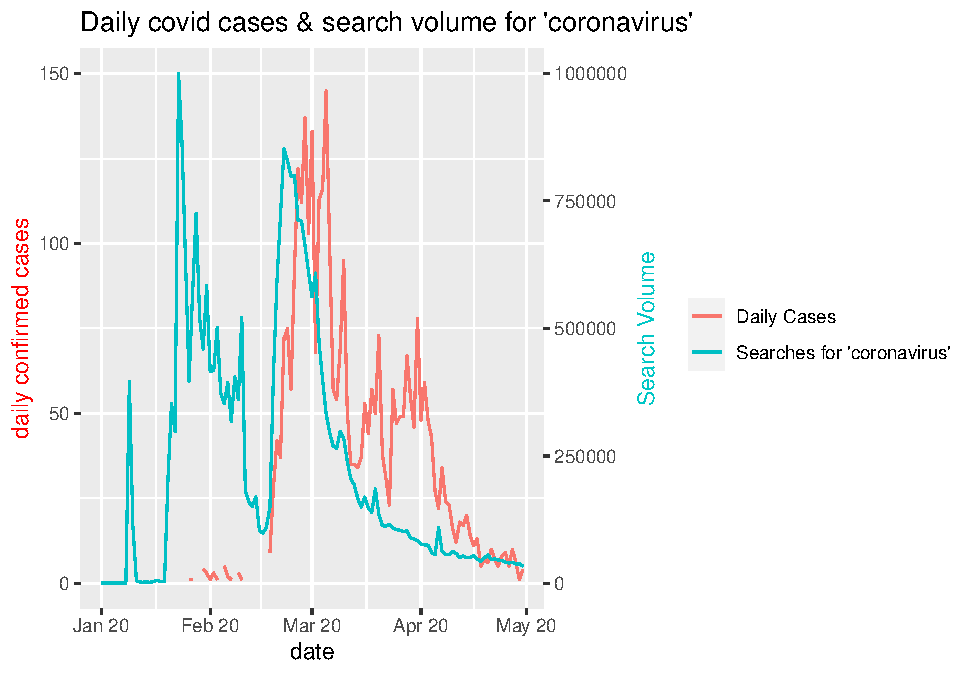
\includegraphics{Main_Analysis_files/figure-latex/unnamed-chunk-5-1.pdf}

~

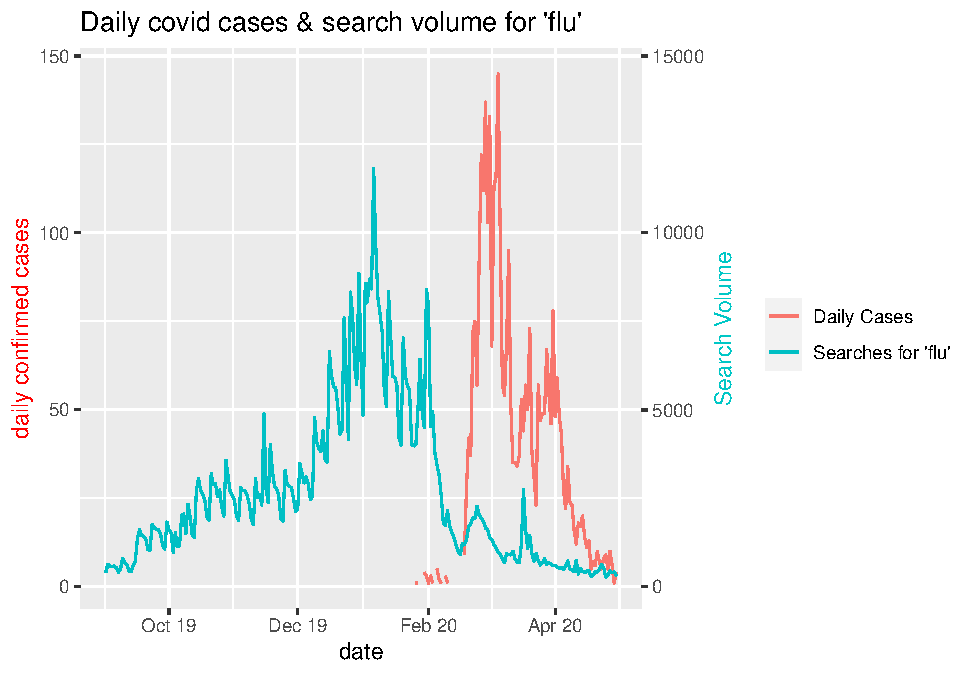
\includegraphics{Main_Analysis_files/figure-latex/unnamed-chunk-6-1.pdf}

~

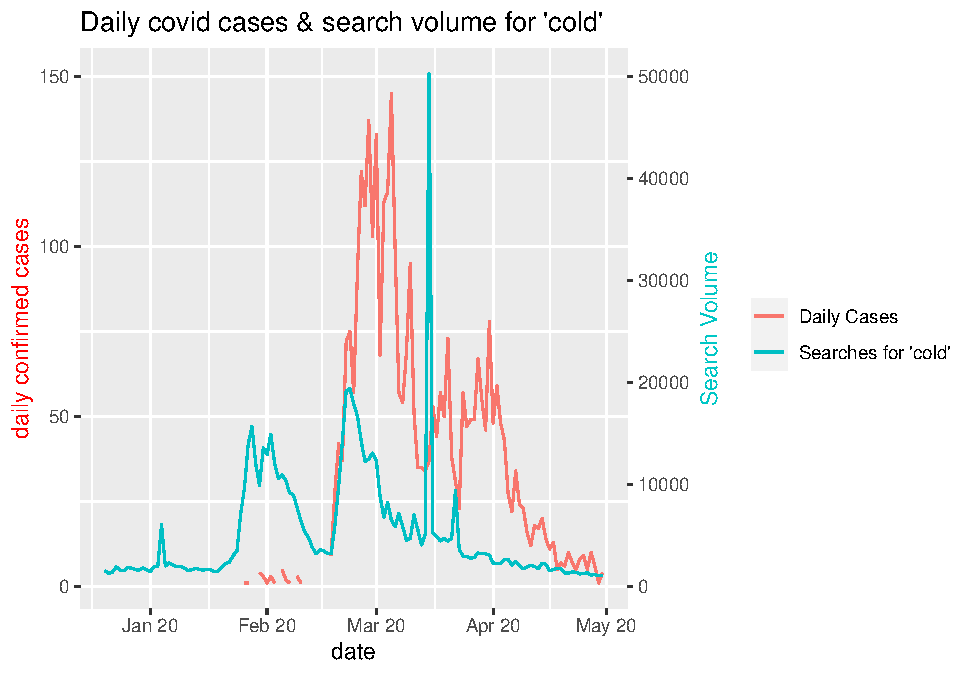
\includegraphics{Main_Analysis_files/figure-latex/unnamed-chunk-7-1.pdf}

\textbf{Short Analysis}

\begin{itemize}
\tightlist
\item
  The term ``coronavirus'' was searched many times more often in
  comparison to the other two available search terms ``flu'' and
  ``cold''.
\item
  Both the search term ``coronavirus'' and ``cold'' show partial
  similarity in its course with the daily confirmed cases (e.g.~strong
  increase in mid-February).
\item
  The gradual increase of the search term ``flu'' starting in October
  2019 could be an indicator of the first (not-tested) covid cases. But
  there is further investigation needed to differentiate the data from
  the annual flu-season.
\end{itemize}

~

\hypertarget{claim-02}{%
\subsection{Claim 02}\label{claim-02}}

\hypertarget{strict-lockdown-measures-have-prevented-a-thorough-spread-in-south-korea.}{%
\paragraph{Strict lockdown measures have prevented a thorough spread in
South
Korea.}\label{strict-lockdown-measures-have-prevented-a-thorough-spread-in-south-korea.}}

\textbf{Our initial motivation:}

\begin{itemize}
\tightlist
\item
  After a massive increase in daily cases, it appears that the
  government of South Korea was able to reduce the number of daily cases
  remarkably within a few days and continued to retain a constant low
  level.
\end{itemize}

\textbf{Claim description in more detail:}

\begin{itemize}
\tightlist
\item
  Stricter lockdown measures lead to a lower outbreak of the Covid-19
  Virus.
\item
  Compared to other countries, for example Germany, the government of
  South Korea reacted more effectively and efficiently.
\end{itemize}

\textbf{Our approach:}

\begin{itemize}
\tightlist
\item
  We first compared the daily cases of South Korea with the ones of
  Germany.
\item
  Next we looked at the different types of government policy measures.
\item
  Within each type of policy we analyzed the different measures in terms
  of time to daily cases.
\end{itemize}

~

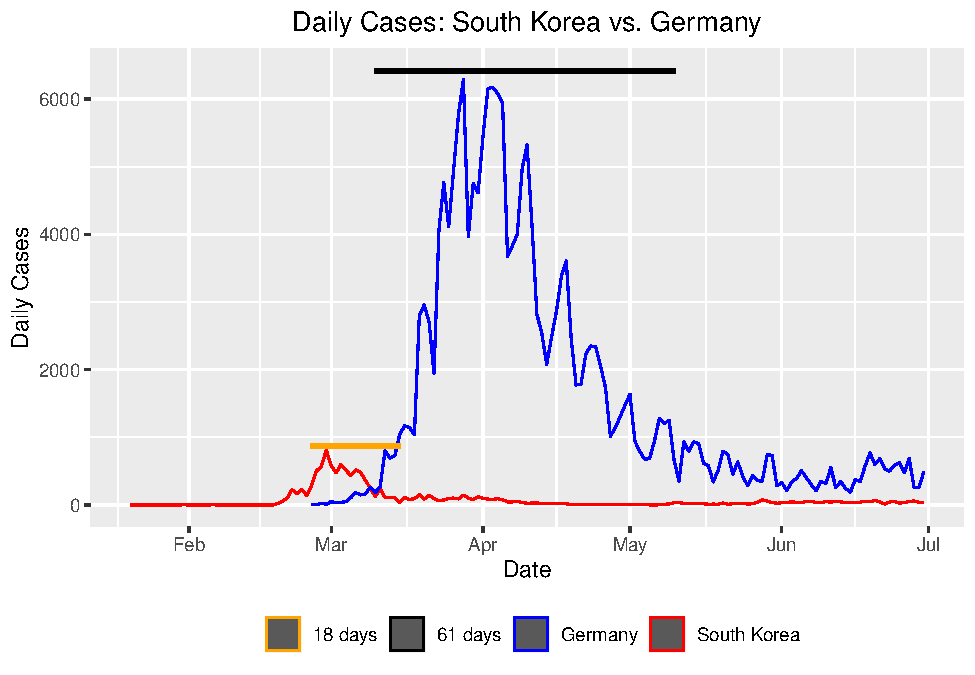
\includegraphics{Main_Analysis_files/figure-latex/unnamed-chunk-9-1.pdf}

\textbf{Short Analysis}

\begin{itemize}
\tightlist
\item
  The total number of daily cases in South Korea compared to Germany is
  considerably lower. Considering the population of each
  country(\textasciitilde50 Mio. vs.~80 Mio.) this seems to be an
  outstanding achievement.
\item
  Compared to Germany, it seems that South Korea needed less time to
  reduce and control the number of daily cases after the first outbreak
  of the virus. It took Germany about three times as long as South Korea
  to get the number of daily cases to a low level again.
\end{itemize}

~

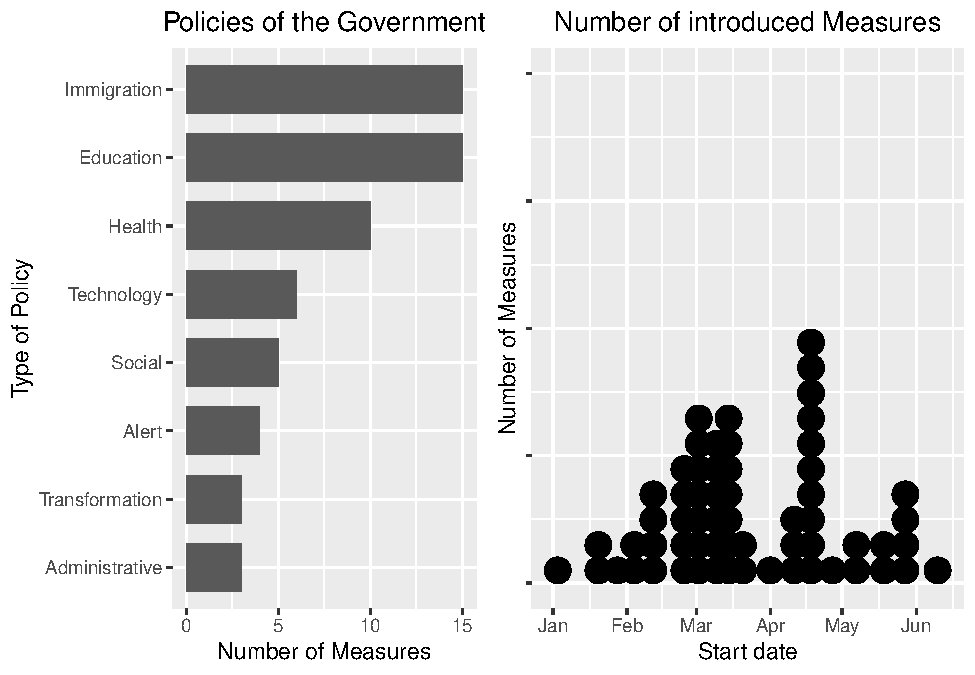
\includegraphics{Main_Analysis_files/figure-latex/unnamed-chunk-10-1.pdf}

\textbf{Short Analysis}

\begin{itemize}
\item
  The number of immigration and education policies dominate the other
  measures. This is related to the fact that immigration measures are
  counted for each country and education measures for each school type.
\item
  Shortly after the number of infection cases surged the government of
  South Korea reacted with numerous measures in all kind of area. The
  many measures in the middle of April are related to the Online-school
  opening measures that all took place at once for each type of school.
\end{itemize}

~

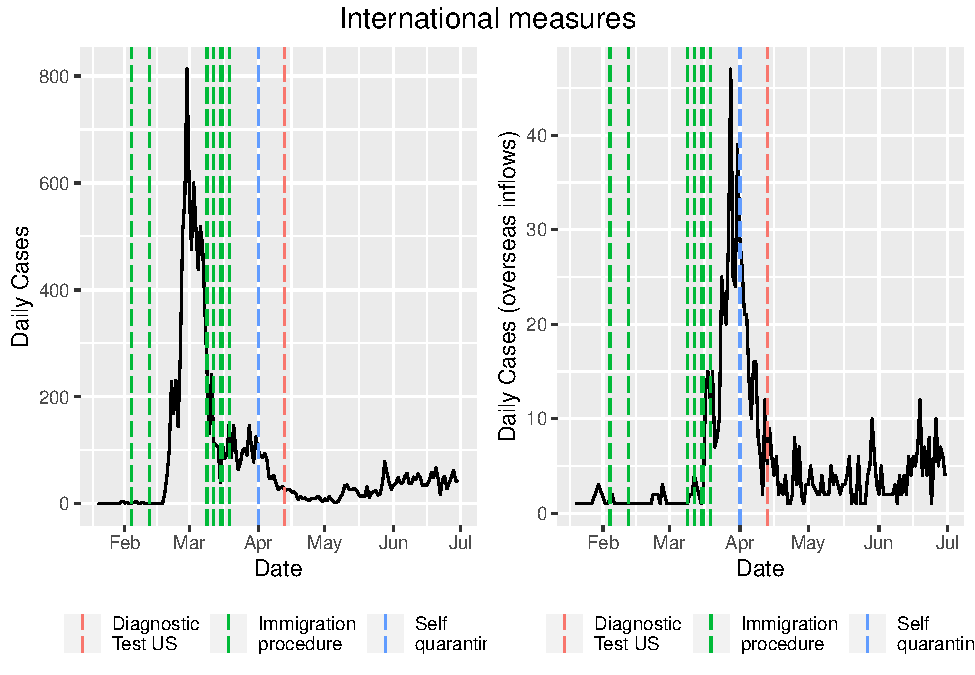
\includegraphics{Main_Analysis_files/figure-latex/unnamed-chunk-13-1.pdf}

\textbf{Short Analysis}

\begin{itemize}
\tightlist
\item
  After experiencing a peak in numbers, the government of South Korea
  established special immigration procedures for foreign countries in
  order to prevent another severe increase in numbers caused by people
  entering the country. However, one can note that shortly afterwards
  the number of daily cases related to overseas inflow first increased
  before plunging afterwards.
\item
  After the number of daily cases related to overseas inflow reached a
  very high level, the government of South Korea imposed a mandatory
  14-day Self-Quarantine. It seems that after a short time the number of
  daily cases related to overseas inflow could be reduced sharply and
  retained a relatively stable level.
\end{itemize}

~

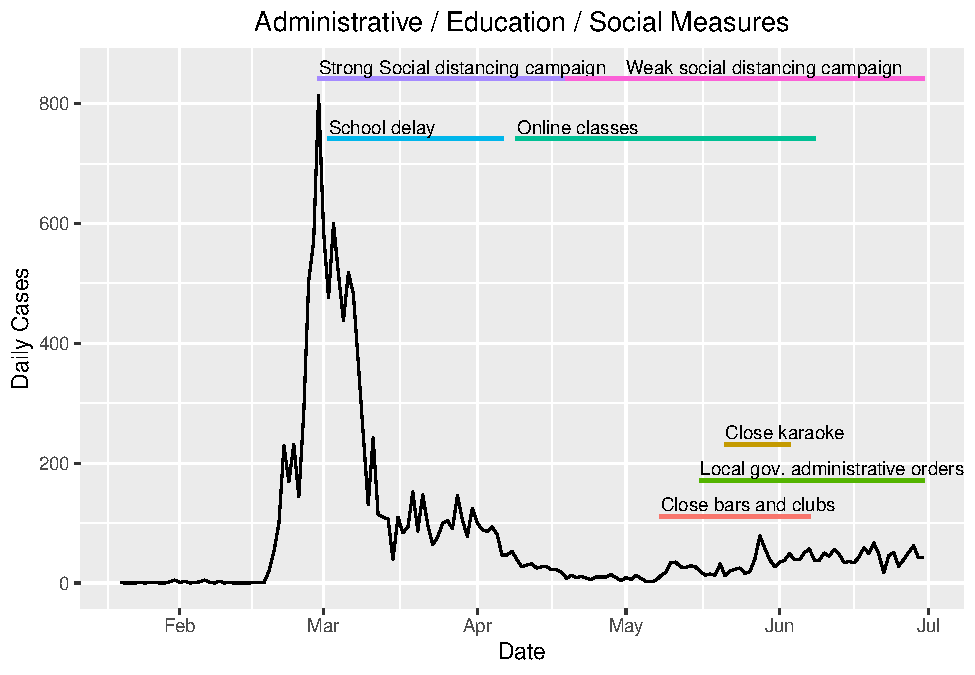
\includegraphics{Main_Analysis_files/figure-latex/unnamed-chunk-14-1.pdf}

\textbf{Short Analysis}

\begin{itemize}
\tightlist
\item
  After the number of daily cases have reached peak in March, numerous
  meausures with the aim of social distancing, such as delaying school
  start, were introduced. It seems that through these measures the
  number of daily cases could be reduced.
\item
  In the beginning of May, after the number of daily cases tended to
  increase again, further public indoor gathering places were forced
  closed. It seems that through that another severe outbreak was
  prevented.
\end{itemize}

~

\hypertarget{claim-03}{%
\subsection{Claim 03}\label{claim-03}}

\hypertarget{superspreader-events-were-the-reason-the-covid-cases-in-south-korea-turned-out-to-be-so-intense-in-the-first-place.}{%
\paragraph{Superspreader Events were the reason the Covid cases in South
Korea turned out to be so intense in the first
place.}\label{superspreader-events-were-the-reason-the-covid-cases-in-south-korea-turned-out-to-be-so-intense-in-the-first-place.}}

\textbf{Our initial motivation:}

\begin{itemize}
\tightlist
\item
  When Covid first reach South Korea the number of cases was relatively
  low. However, with the ``mysterious'' patient Number 31, the serious
  increase in daily cases in South Korea began. A lot ot people
  worldwide including the local government blamed a Christian `Cult' for
  this, since one member seemed to have spread the virus.
\end{itemize}

\textbf{Claim description in more detail:}

\begin{itemize}
\tightlist
\item
  Without this particular spreader event in the Shincheonji Church in
  Daegu the Covid-spread would have been seriously lower.
\item
  In fact, one could argue that without those spreader events the
  Covid-spread in South Korea wouldn't have been ``serious'' at all.
\end{itemize}

\textbf{Our approach:}

\begin{itemize}
\tightlist
\item
  In order to see, whether the public media was right, and the Church
  did indeed cause the first ``serious'' spread of the virus we first
  had a look at the most common reasons for a Covid infection within
  South Korea.
\item
  We then created a graph showing the daily cases related to the main
  spreader events in comparison to the overall daily cases.
\item
  Finally, we created a first map of South Korea showing the outbreaks
  in the different regions together with the specific locations of the
  different spreader events.
\end{itemize}

\hypertarget{first-part-of-the-analyis}{%
\paragraph{First part of the analyis}\label{first-part-of-the-analyis}}

\textbf{Who was infected by with infection case? What role do the super
spreader events play?}

~

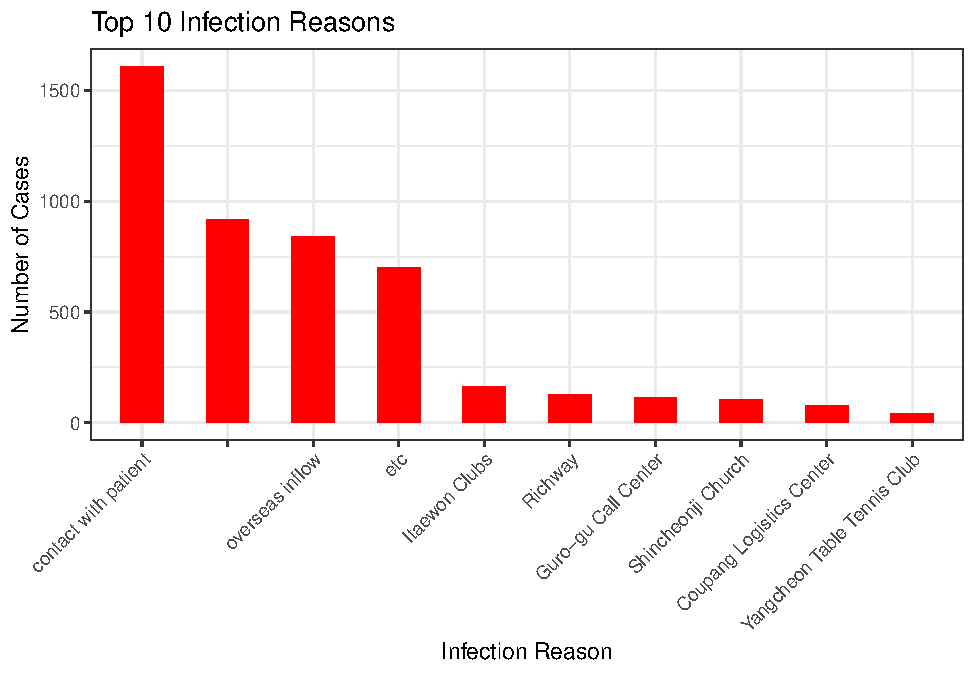
\includegraphics{Main_Analysis_files/figure-latex/unnamed-chunk-15-1.pdf}

\textbf{Short Analysis:}

\begin{itemize}
\tightlist
\item
  Seems like apart from contact with a patient and oversees inflow, the
  main reasons for getting Covid-19 were related to some main events
  that happened throughout the country.
\item
  The most cases are related to the Itaewon clubs. The church that we
  read about in the news is on 4th place when we don't count contact
  with patient, overseas inflow etc.
\end{itemize}

\begin{center}\rule{0.5\linewidth}{0.5pt}\end{center}

Following, we'll create a graph comparing the total daily cases with the
daily cases related to the super spreader events. Since the
``patientinfo'' table represents only a sample of the total amount of
cases, we will first show, that patientinfo can indeedn be seen as a
representative sample of the total amount of cases.

~

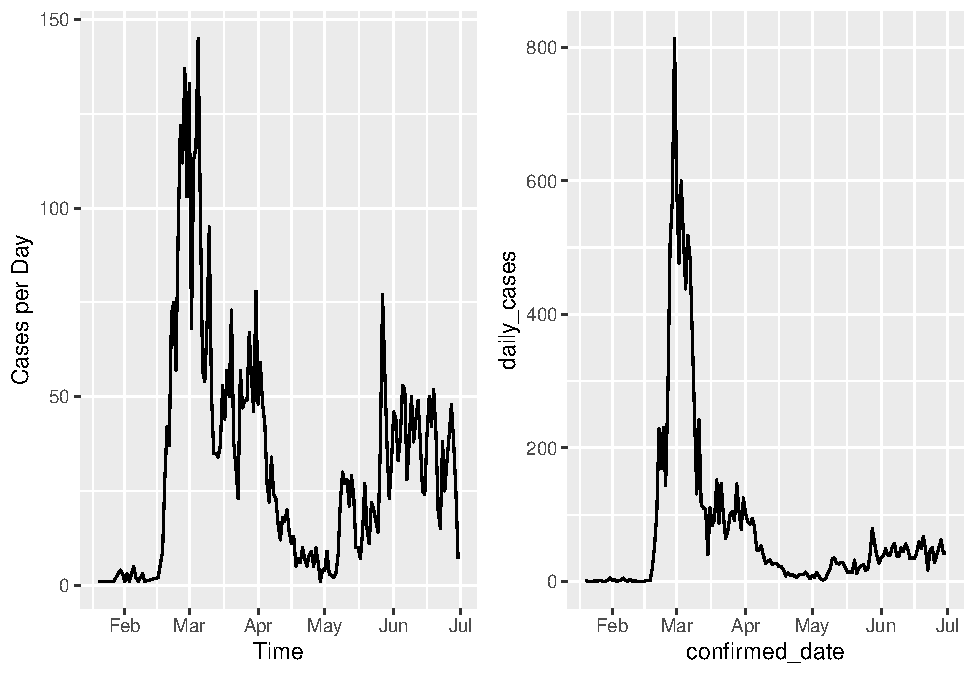
\includegraphics{Main_Analysis_files/figure-latex/unnamed-chunk-16-1.pdf}

As one can see both graph lines follow a similar pattern over the same
time period. Therefore, we will assume that we can treat patientinfo as
a representative sample.

~

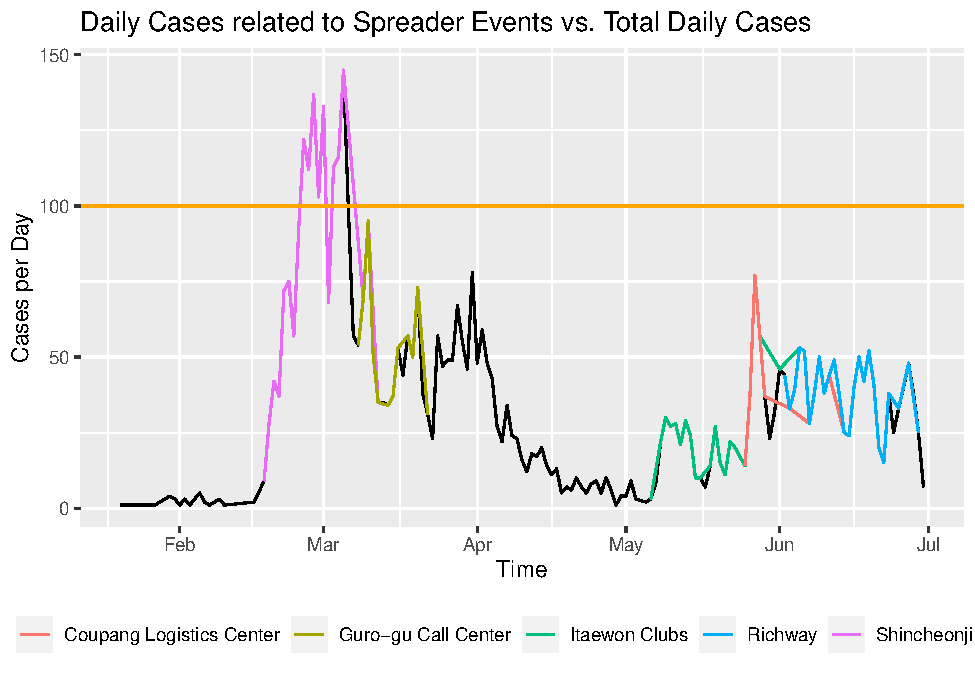
\includegraphics{Main_Analysis_files/figure-latex/unnamed-chunk-17-1.pdf}

\textbf{Short Analysis:}

\begin{itemize}
\tightlist
\item
  The different spreader events match the daily cases over time pretty
  well!
\item
  Especially the first event (the Church!) shows that when cases
  exploded, a whole lot was related to the church everyone is blaming.
\item
  Let's see when exactly the main event happened and match only the
  first event with overall cases.
\end{itemize}

~

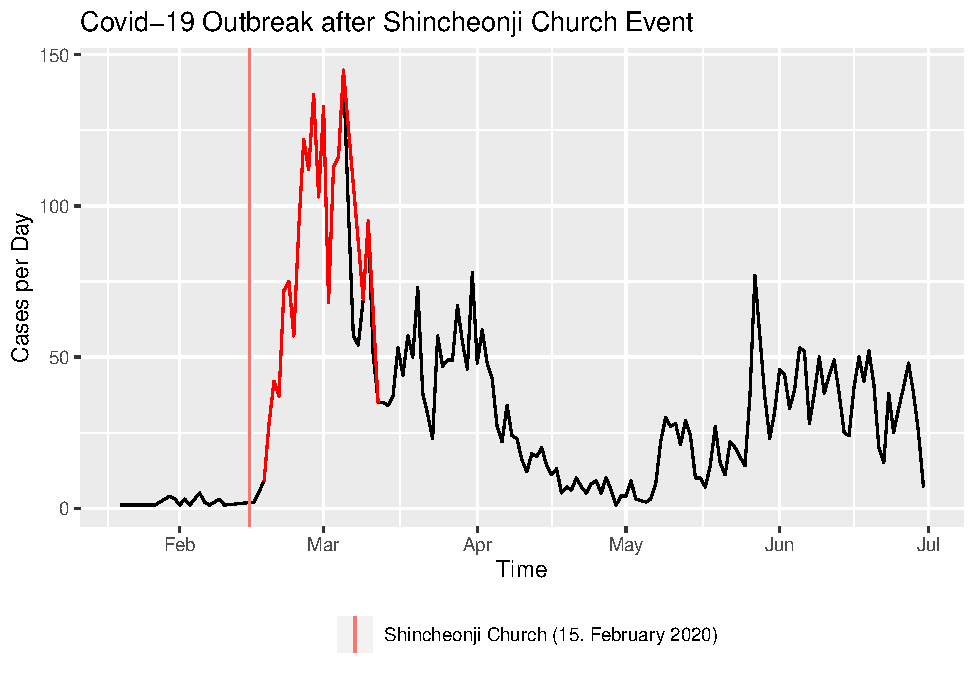
\includegraphics{Main_Analysis_files/figure-latex/unnamed-chunk-18-1.pdf}

\textbf{Short Analysis}

\begin{itemize}
\tightlist
\item
  This matches pretty well.
\item
  Of course we need to take into account that the ``real'' amount of
  daily cases goes up to 800 so the almost 150 daily cases at this one
  day in March connected to the Church are not the total number of cases
  that day.
\item
  Still, the impact the church outbreak had on the whole Covid situation
  in South Korea is pretty intense.
\end{itemize}

~

\hypertarget{second-part-of-the-analyis}{%
\paragraph{Second part of the
analyis}\label{second-part-of-the-analyis}}

\textbf{Where exactly did the events take place? Are we able to see a
connection between large outbreaks and the Spreader events?}

~

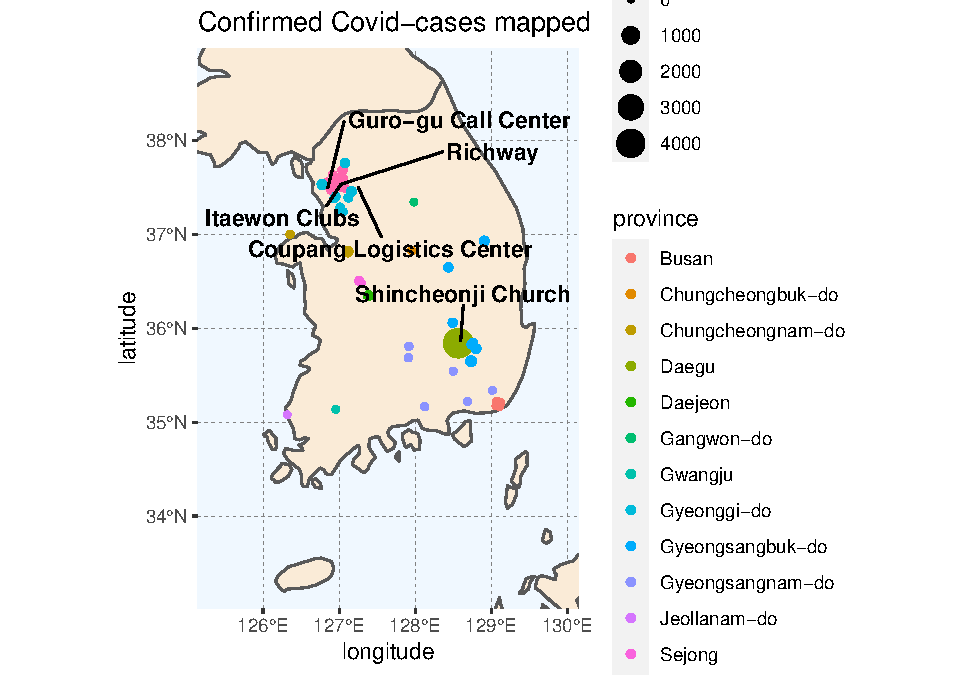
\includegraphics{Main_Analysis_files/figure-latex/unnamed-chunk-20-1.pdf}

\textbf{Short Analysis:}

\begin{itemize}
\tightlist
\item
  One can clearly see the connection between large outbreak locations
  and the spreader events. While multiple cases and events occurred in
  Seoul (North-West part of South Korea), the most interesting thing is
  the very first spreader event in Daegu (Shincheonji Church).
\item
  Interesting is as well, that his map shows not only part of the acutal
  cases (such as the Patientinfo table) but a real overview of the
  number of cases occurred in the different areas.
\item
  Thus, one can clearly see the influence the main first spreader event
  in the Shincheonji Church in Daegu had. One could argue that without
  the event the cases might have been seriously lower. However, further
  analysis would have had to be conducted in order to confirm this.
\end{itemize}

\end{document}
